%%%%%%%%%%%%%%%%%%%%%%%%%%%%%%%%%%%%%%%%%%%%%%%%%%%%%%%%%%%%%%%%%%%%%%
\subsection{Matlab und Octave}
\frame{\subtoc}

\begin{frame}
  Matlab und Octave sind beides große Programmpakete mit einer auf die
  Lösung mathematischer Aufgaben fokussierten Programmiersprache.

  Beide Programmiersprachen sind weitgehend kompatibel miteinander.

  \begin{columns}
    \begin{column}[t]{.49\textwidth}
      \begin{block}{Matlab}
        \begin{itemize}
        \item Kommerzielle Software
        \item Studierendenlizenzen im URZ
        \item Besser auf Leistung optimiert
        \item Besseres GUI
        \end{itemize}
      \end{block}
    \end{column}
    \begin{column}[t]{.49\textwidth}
      \begin{block}{GNU Octave}
        \begin{itemize}
        \item Freie Software
        \item Sehr gut für uns geeignet
        \item Besserer DGL-Löser?
        \end{itemize}
      \end{block}
    \end{column}
  \end{columns}
\end{frame}

\begin{frame}{Downloading}

  \begin{itemize}
  \item GNU Octave
    \begin{itemize}
    \item The homepage is \url{https://octave.org/}
    \item The direct download link is \url{https://octave.org/download.html}
    \end{itemize}
  \item Matlab
    \begin{itemize}
    \item
      \url{https://www.urz.uni-heidelberg.de/de/service-katalog/software-und-anwendungen/matlab-simulink}
    \end{itemize}
  \end{itemize}
\end{frame}

\begin{frame}{lsode (Octave)}
  Die Funktion \lstinline!lsode(@fun, x0, tinv)! löst
  \begin{gather*}
    x' = \text{fun}(x,t), \qquad x(t_0) = x0.
  \end{gather*}
  Sie hat 3 Parameter:
  \begin{enumerate}
  \item \lstinline!@fun! ist die rechte Seite der Gleichung als Funktion
  \item \lstinline!x0! ist der Startwert, immer als Vektor
  \item \lstinline!tinv! ist ein Vektor mit allen Zeitpunkten, an denen
    die Lösung gewünscht ist
  \end{enumerate}
  Der Rückgabewert ist ein Vektor mit einer Lösung für jeden Eintrag
  von \lstinline!tinv!
\end{frame}

\begin{frame}{Beispielprogramm (lsode)}
  \lstinputlisting{octave/logistic.m}

  \lstinputlisting{octave/simple_lsode.m}
\end{frame}

\begin{frame}{ode45 (Matlab, Octave)}
  Die Funktion \lstinline!ode45(@fun, tinv, x0)! löst
  \begin{gather*}
    x' = \text{fun}(t,x), \qquad x(t_0) = x0.
  \end{gather*}
  Sie hat 3 Parameter:
  \begin{enumerate}
  \item \lstinline!@fun! ist die rechte Seite der Gleichung als Funktion
  \item \lstinline!tinv = [t0,tend]! ist das Zeitintervall
  \item \lstinline!x0! ist der Startwert, immer als Vektor
  \end{enumerate}
  Die Funktion gibt einen Vektor mit Zeitpukten und einen mit
  Funktionswerten zurück.
\end{frame}

\begin{frame}{Beispielprogramm (ode45)}
  \lstinputlisting{octave/logistic_ode45.m}

  \lstinputlisting{octave/simple_ode45.m}
\end{frame}



%%%%%%%%%%%%%%%%%%%%%%%%%%%%%%%%%%%%%%%%%%%%%%%%%%%%%%%%%%%%%%%%%%%%%%
\subsection{Fehler und Berechenbarkeit}
\frame{\subtoc}

\begin{frame}{Fehlerquellen bei der Simulation einer AWA}
  \begin{enumerate}
  \item Messfehler
    \begin{itemize}
    \item Startwerte
    \item Funktionsparameter
    \end{itemize}
  \item Modellfehler
    \begin{itemize}
    \item vernachlässigte Mechanismen
    \item indirekt gemessene Funktionsparameter
    \end{itemize}
  \item Diskretisierungsfehler
    \begin{itemize}
    \item Ersatz der DGl durch ein Zeitschrittverfahren
    \end{itemize}
  \item Rechenfehler
    \begin{itemize}
    \item Rundung bei der Zahlendarstellung im Computer
    \item Inexakte Berechnungen im Algorithmus
    \end{itemize}
  \end{enumerate}
\end{frame}

\begin{frame}{Modellierung von Mess- und Modellfehler}
  \begin{xalignat*}2
    \text{tatsächlich:}\qquad x' &= f(x,t) & x(0) &= x_0\\
    \text{Modell:}\qquad y' &= g(y,t) & y(0) &= y_0
  \end{xalignat*}
  Für ein kleines Teilintervall mit Startwerten $x_0,y_0$ setzt sich der Fehler $y(t)-x(t)$ am Ende aus 3 Komponenten zusammen:
  \begin{enumerate}
  \item Differenz $y(0)-x(0)$ am Anfang
  \item Differenz $g(y,t) - f(y,t)$ im Intervall
  \item Differenz $f(y,t) - f(x,t)$ im Intervall
  \end{enumerate}
\end{frame}

\begin{frame}{Fehlerdarstellung}
  \begin{gather*}
    y(t)-x(t) = y_0-x_0
    + \int_0^t \bigl[
    g(y(s),s) - f(x(s),s)\bigr] \,ds
  \end{gather*}
  \pause
  Ergänzen einer null
  \begin{gather*}
    y(t)-x(t) = y_0-x_0
    + \int_0^t \bigl[
    g(y(s),s) - f(y(s),s)\bigr] \,ds
    + \int_0^t \bigl[
    f(y(s),s) - f(x(s),s)\bigr] \,ds
  \end{gather*}
  \begin{enumerate}
  \item Anfangswertfehler
  \item Modellfehler
  \item Fortpflanzung des Anfangswertfehlers
  \end{enumerate}
\end{frame}

\begin{frame}{Beispiel}
  \begin{xalignat*}3
     x' &= 2x & x(0) &= 3 & x(t) &= 3e^{2t}\\
    y' &= 2.1y & y(0) &= 3.1 & y(t) &= 3.1 e^{2.1t}
%    \only<2->{z' &= 2z & z(0) &= 3.1 & z(t) &= 3.1 e^{2t}}
  \end{xalignat*}
  \small
  \begin{alignat*}2
    \int_0^t \bigl[g(y(s))-f(y(s))\bigr] &= \int_0^t 0.31 e^{2.1s} &&= \tfrac{0.31}{2.1}\bigl(e^{2.1t}-1\bigr)
    \\
    \int_0^t \bigl[f(y(s))-f(x(s))\bigr] &= \int_0^t 2(3.1e^{2.1s} - 3e^{2s}) &&= \tfrac{6.2}{2.1}\bigl(e^{2.1t}-1\bigr) - 3\bigl(e^{2t}-1\bigr)
  \end{alignat*}
  \begin{columns}
    \begin{column}{.7\textwidth}
      \begin{gather*}
        \begin{aligned}
          x(1) &= 3e^2 &&= 22.167\\
          y(1) &= 3.1e^{2.1} && = 25.315\\
        \end{aligned}\\
        y(1)-x(1) = 0.1+ 1.0579 + 1.9901 = 3.1480
  \end{gather*}      
    \end{column}
    \begin{column}{.3\textwidth}
      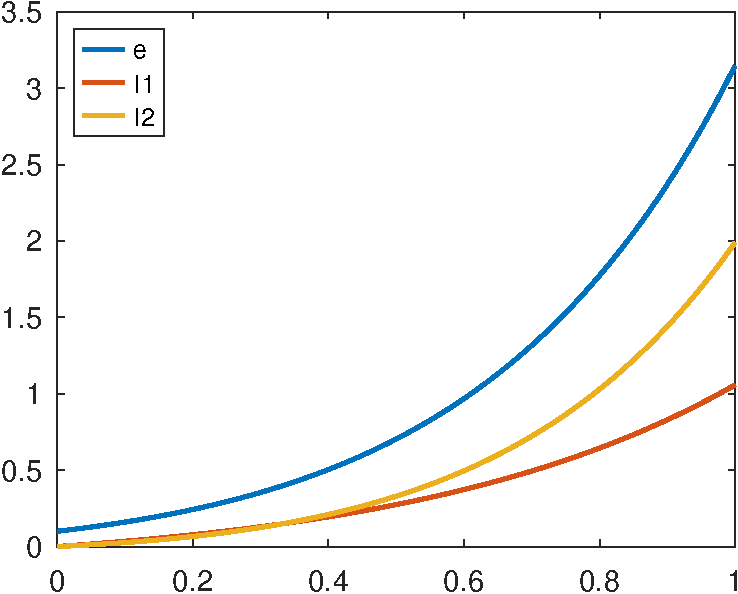
\includegraphics[width=\textwidth]{fig/error-simple-crop.pdf}
    \end{column}
  \end{columns}
\end{frame}

\begin{frame}{Diskussion}
  Der Fehler des Startwerts 0.1 zum Zeitpunkt $t=0$ hat sich zu $t=1$ auf
  3.148 erhöht.

  \vspace{1cm}
  
  \only<1>{
    \begin{exampleblock}{Frage}
      Ist das nicht ein katastrophales, unnützes Ergebnis?
    \end{exampleblock}
  }
\end{frame}

\begin{frame}[fragile]
\begin{block}{Definition}
    Wir für die Differenz zwischen der exakten Lösung $x$ einer
    Aufgabe und einer Approximation $y$ führen wir folgende Fehlermaße
    ein:
    \begin{align*}
      \text{absoluter Fehler:}& \norm{y-x}\\
      \text{relativer Fehler:}& \frac{\norm{y-x}}{\norm x}.      
    \end{align*}
    Die Doppelstriche $\norm\cdot$ bezeichnen eine Norm im
    $\mathbb R^n$ oder den Absolutbetrag in einer Dimension.
  \end{block}
  \begin{gather*}
    \begin{array}{cccc}
    %   t & x & \norm{y-x} & \frac{\norm{y-x}}{\norm x}
    %   \\\hline
    %   0 & 3 & 0.1 & 0.0333\\
    %   1 & 22.167 & 3.148 & 0.142
    \end{array}
  \end{gather*}
\end{frame}

\begin{frame}{Schranken für die Fehlerterme}
  Mess- und Modellierungsfehler seien aus der Anwendung bekannt,
  \begin{align*}
    \norm{y_0-x_0} &\le E_0\\
    \norm{g(y,t)-f(y,t)} &\le E_1 \quad\text{für alle relevanten $(y,t)$}
  \end{align*}
  $E_1$ darf hierbei auch von $t$ abhängen,
  \pause
  \begin{block}{Lipschitzbedingung}
    Für alle relevanten $x,y,t$ gelte
    \begin{gather*}
      \norm{f(y,t) - f(x,t)} \le L \norm{y-x}.
    \end{gather*}
  \end{block}
\end{frame}

\begin{frame}{Was ist relevant?}
  \begin{itemize}
  \item In der mathematischen Formulierung finden Sie Ausdrücke, die
    zu korrekten Resultaten führen, aber eventuell nicht erfüllbar
    sind.
  \item Oft ist bekannt, dass die Lösungen beschränkt sind, was die
    Menge der relevanten Punkte einschränkt.
  \end{itemize}
  \pause
  Beispiele:
  \begin{itemize}
  \item Gelten die Abschätzungen für alle $t\in \R$ und $x,y\in \R^n$,
    so sind wir fertig.
    \pause
  \item Wenn bekannt ist, dass die Lösungen beschränkt sind, dann
    genügt oft $\norm x, \norm y < r$.
  \item Für $t$ müssen nur Werte im Zeitintervall von Interesse
    beachtet werden.
  \end{itemize}
\end{frame}

\begin{frame}
  Sei $e(t) = y(t)-x(t)$. Es gilt dann
  \begin{gather*}
    \norm{e(t)} = \underbrace{\norm{e(0)}}_{\le E_0}
    + \int_0^t \underbrace{\bigl[
      g(y,s) - f(y,s)\bigr]}_{\le E_1(s)} \,ds
    + \int_0^t \underbrace{\bigl[
      f(y,s) - f(x,s)\bigr]}_{\le L \norm{y-x}} \,ds
  \end{gather*}
  daher gilt
  \begin{gather*}
    \norm{e(t)}\le E_0 + \int_0^t L \norm{e(s)}\,ds
    +\int_0^t E_1(s)\,ds
  \end{gather*}

  \begin{block}{Fehlerabschätzung}
    Es gelten die angegebenen Schranken für die Fehlerterme, besonders
    die Lipschitzbedingung. Dann gilt
    \begin{gather*}
       \norm{e(t)}\le e^{Lt} \left[ E_0+\int_0^t E_1(s)\,ds\right]
    \end{gather*}
  \end{block}
\end{frame}

\begin{frame}{Beispiel}
  \begin{xalignat*}3
    x' &= 2x & x(0) &= 3 & x(t) &= 3e^{2t}\\
    y' &= 2y & y(0) &= 3.1 & y(t) &= 3.1 e^{2t}
  \end{xalignat*}
  Es ist also $E_0 = 0.1$, $E_1 = 0$ und $L=2$. Unsere Abschätzung ergibt
  \begin{gather*}
    \norm{e(t)} \le 0.1 e^{2t},
  \end{gather*}
  was in diesem Falle sogar exakt ist. Für den relativen Fehler gilt
  \begin{gather*}
    \frac{\norm{e(t)}}{\norm{x(t)}} \le 0.0334.
  \end{gather*}  
\end{frame}

\begin{frame}{Negatives Beispiel}
  \begin{xalignat*}3
    x' &= -2x & x(0) &= 3 & x(t) &= 3e^{-2t}\\
    y' &= -2y & y(0) &= 3.1 & y(t) &= 3.1 e^{-2t}
  \end{xalignat*}
  Es ist noch immer $E_0 = 0.1$, $E_1 = 0$ und $L=2$ und
  \begin{gather*}
    \norm{e(t)} \le 0.1 e^{2t}.
  \end{gather*}
  Für den relativen Fehler gilt
  \begin{gather*}
    \frac{\norm{e(t)}}{\norm{x(t)}} \le 0.0334 e^{4t},
  \end{gather*}
  was bestenfalls nutzlos ist.
\end{frame}

\begin{frame}
  \begin{block}{Einseitige Lipschitzbedingung}
    Für alle relevanten $x,y,t$ gilt
    \begin{gather*}
      \scal({f(y,t)-f(x,t)},y-x) \le \mu \norm{y-x}^2.
    \end{gather*}
  \end{block}

  $\mu$ kann, wie in unserem Beispiel, negativ sein!
  
  \begin{block}{Verbesserte Fehlerabschätzung}
    Es sei der Einfachheit halber $E_1=0$ und es gelte
    die einseitige Lipschitzbedingung. Dann gilt
    \begin{gather*}
       \norm{e(t)}\le  E_0 e^{\mu t}
    \end{gather*}
  \end{block}
\end{frame}

\begin{frame}
  \begin{block}{Bemerkung}
    Die Lipschitzbedingung besagt nichts anderes, als dass es eine
    lineare Differentialgleichung gibt, deren Lösung schneller wächst
    als die der Gleichung mit rechter Seite $f(x,t)$.
  \end{block}
\end{frame}

%%%%%%%%%%%%%%%%%%%%%%%%%%%%%%%%%%%%%%%%%%%%%%%%%%%%%%%%%%%%%%%%%%%%%%
\subsection{Zeitschrittmethoden}
\frame{\subtoc}

\begin{frame}{Das allgemeine Konzept}
  Beginnend mit dem Startwert $\hat x_0 = x_0$ ,an der Stelle $t_0$,
  berechne rekursiv weitere Werte der approximierten Lösung $\hat x_k$ für $k=1,2,\ldots$:
  \begin{align*}
    t_k &= t_{k-1} + h_k\\
    \hat x_k &= \hat x_{k-1} + h_k F_{h_k}(\hat x_{x-1},t_{k-1}).
  \end{align*}
  \begin{itemize}
  \item $h_k$ ist die Schrittweite im Schritt $k$
  \item $F_{h_k}(\hat x_{x-1},t_{k-1})$, so dass allgemein
    \begin{gather*}
      h F_{h}(y,t) \approx \int_t^{t+h} f(y(s),s)\,ds,
    \end{gather*}
    wobei $y(s)$ Lösung der Volterraschen Integralgleichung mit
    Startwert $y$ zum Zeitpunkt $t$ ist.
  \end{itemize}
\end{frame}

\begin{frame}{Beispiel: Eulersches Polygonzugverfahren}
  \begin{gather*}
    x_{k} = x_{k-1} + h_k f(x_{k-1},t_{k-1})
  \end{gather*}
  \begin{center}
    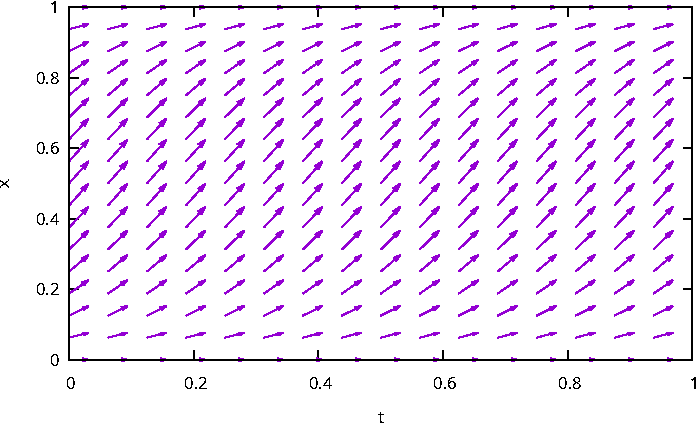
\includegraphics[width=.6\textwidth]{fig/euler-logistic.pdf}
  \end{center}
\end{frame}

\begin{frame}
  \begin{center}
    \only<1>{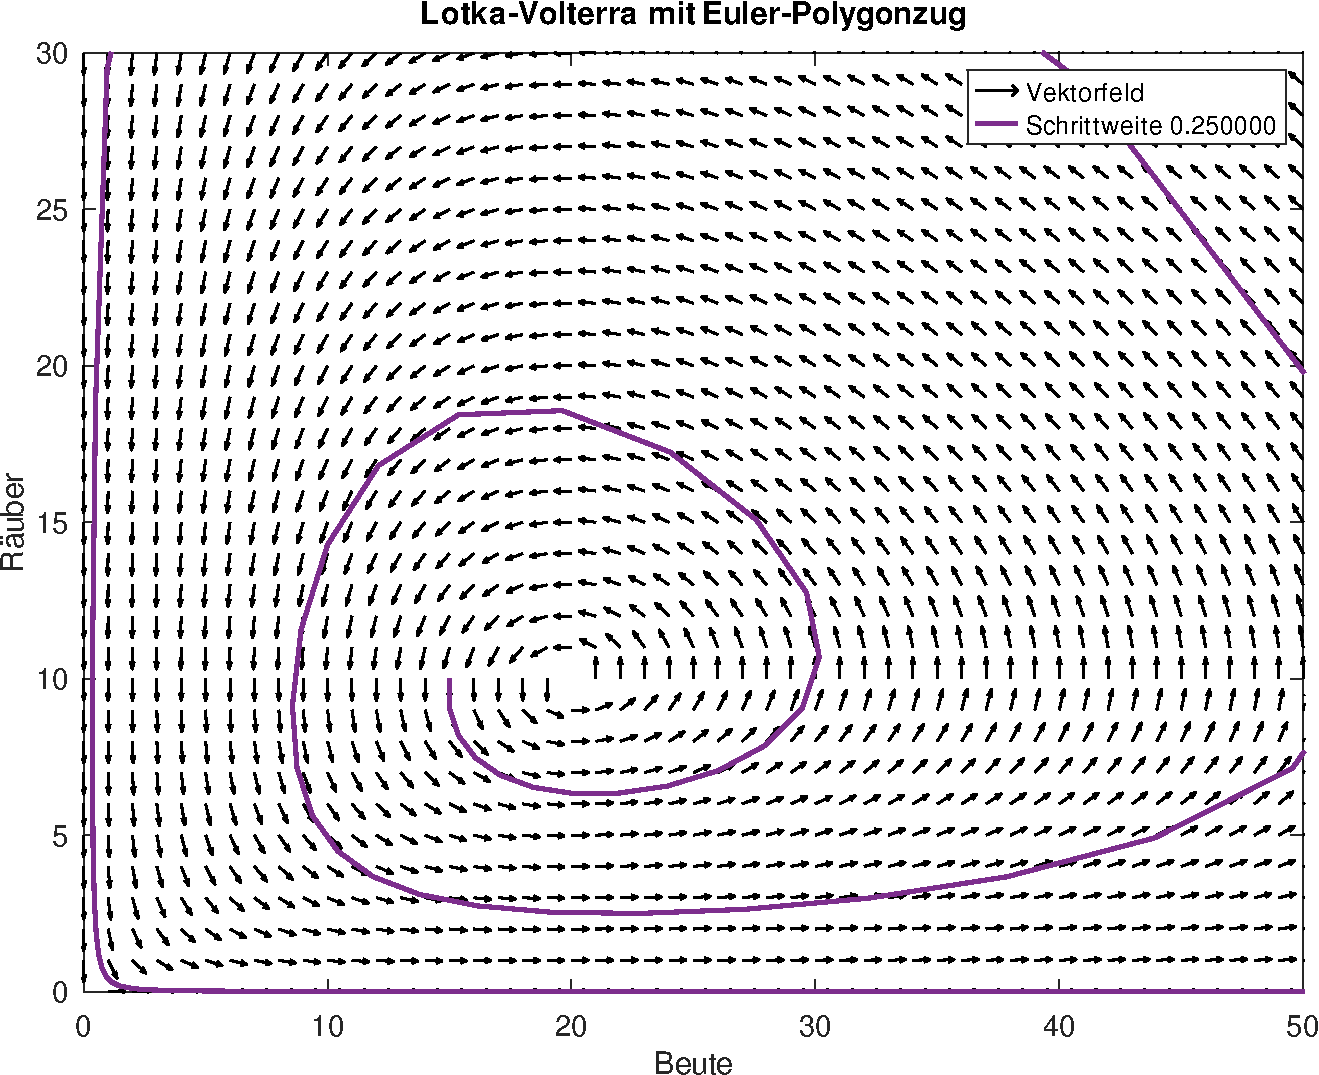
\includegraphics[width=.8\textwidth]{fig/Euler-LV-80-crop.pdf}}
    \only<2>{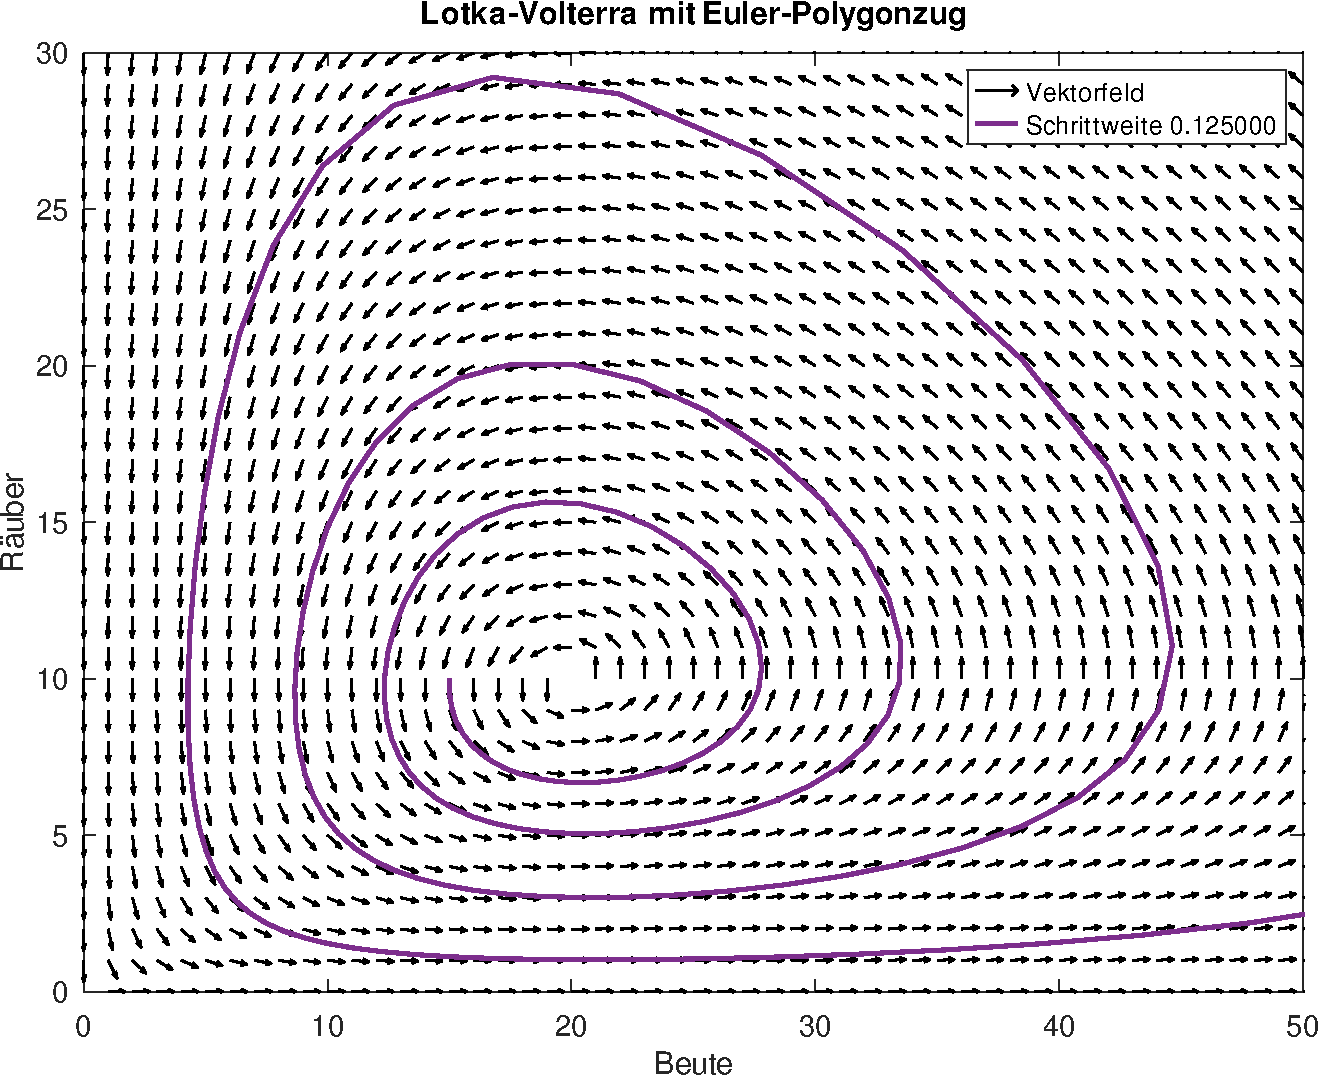
\includegraphics[width=.8\textwidth]{fig/Euler-LV-160-crop.pdf}}
    \only<3>{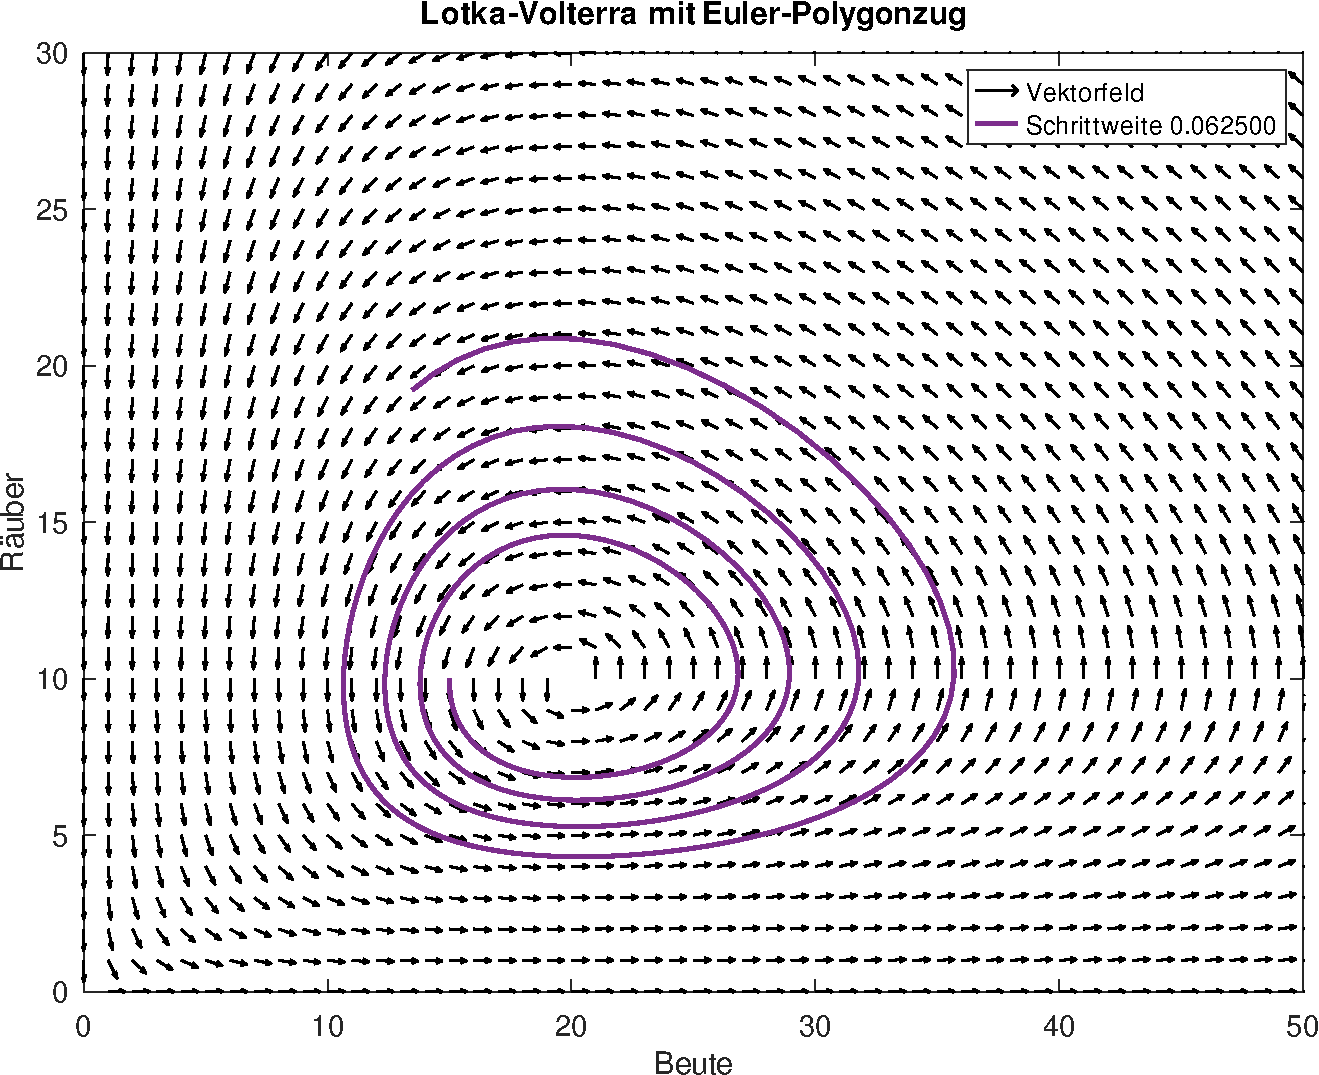
\includegraphics[width=.8\textwidth]{fig/Euler-LV-320-crop.pdf}}
    \only<4>{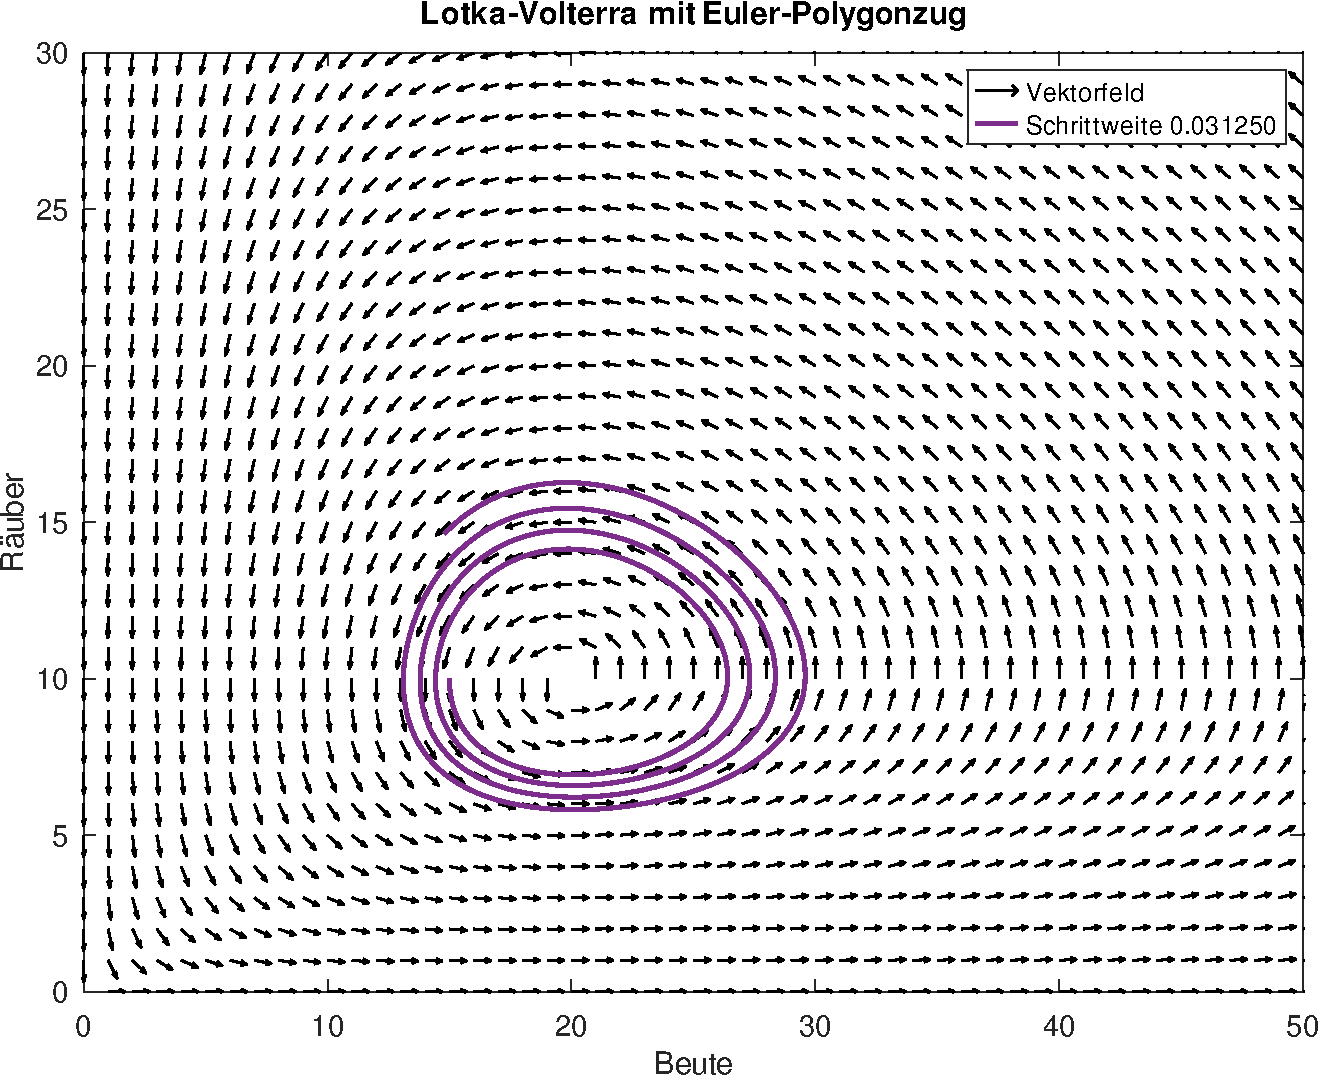
\includegraphics[width=.8\textwidth]{fig/Euler-LV-640-crop.pdf}}
  \end{center}
\end{frame}

\begin{frame}{Beispiel: das \glqq{}klassische\grqq{} Runge-Kutta-Verfahren}
  \begin{xalignat*}2
    && k_1 &= f\left(y,t\right)\\
    y_1 &= y+\tfrac12 hk_1 &  k_2 &= f\left(y_1, t+\tfrac12 h\right)\\
    y_2 &= y+\tfrac12 hk_2 & k_3 &= f\left(y_2, t+\tfrac12 h\right)\\
    y_3 &= y+ hk_3 & k_4 &= f\left(y_3, t+h\right)\\
  \end{xalignat*}
  \vspace{-1.5cm}
  \begin{gather*}
    F_h(y,t) = y+h\left(\tfrac16k_1+\tfrac13k_2+\tfrac13k_3+\tfrac16k_4\right)    
  \end{gather*}
  Die Punkte $y_1,\dots,y_3$ sind Hilfskoordinaten, die ähnlich dem
  Euler-Verfahren konstruiert werden, die Verfahrensfunktion ist dann
  eine geeignete Kombination der Funktionswerte an diesen Punkten.
\end{frame}

\begin{frame}
  \begin{center}
    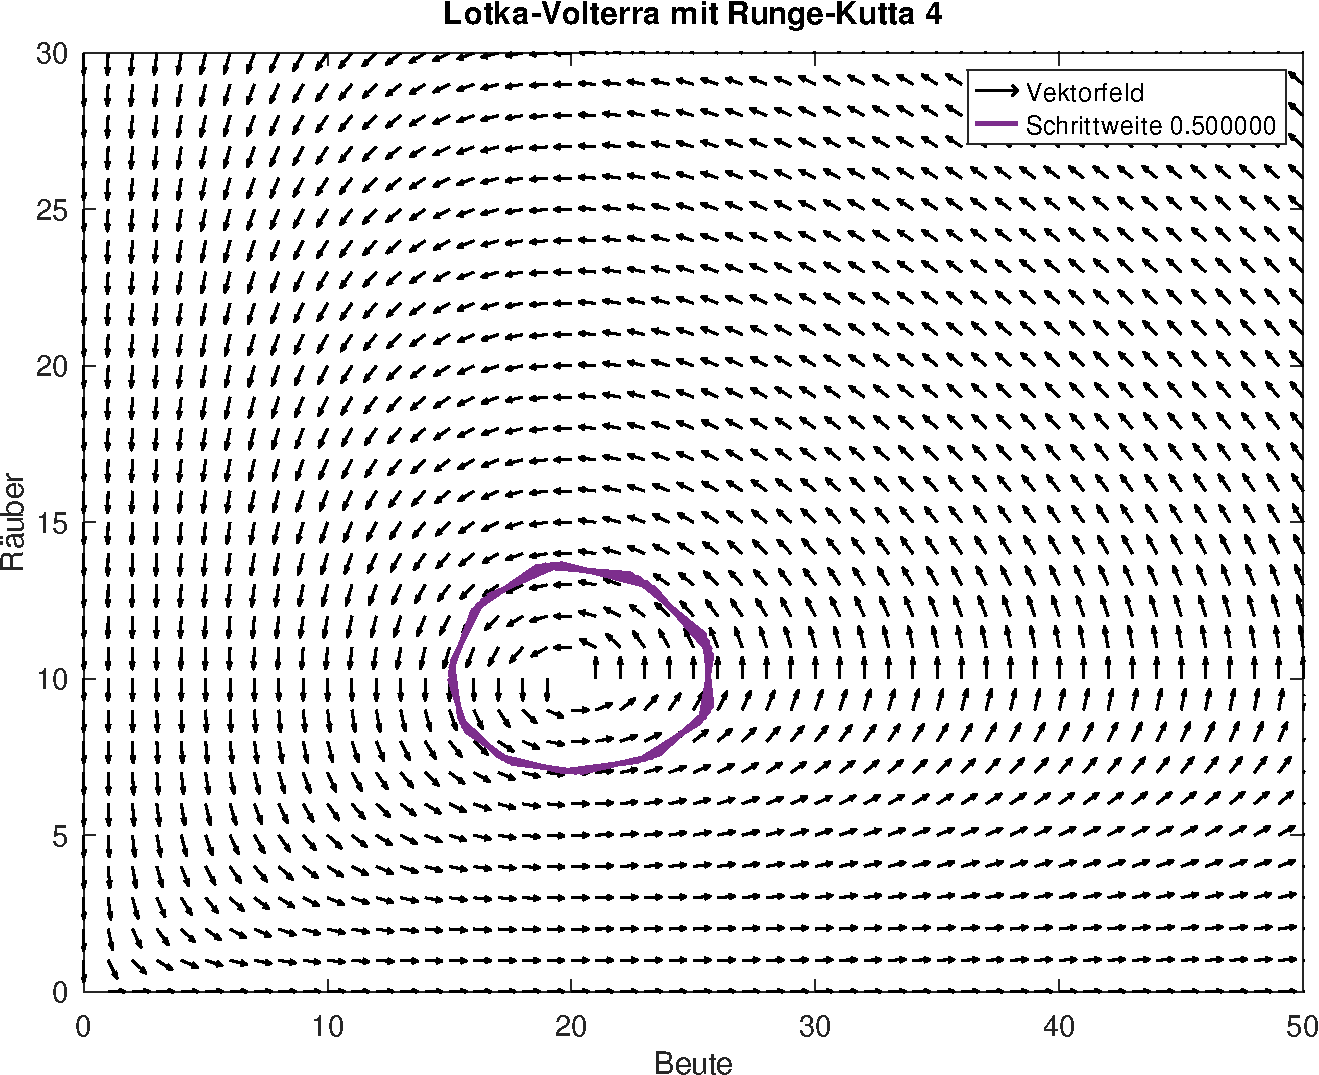
\includegraphics[width=.8\textwidth]{fig/RK4-LV-40-crop.pdf}
  \end{center}
\end{frame}

% \begin{frame}{Fehleranalyse}
%   \begin{block}{Lokaler Fehler}
%     Der lokale Fehler eines Zeitschrittverfahrens ist für Lösungen der
%     Volterraschen Integralgleichung beginnend in $(y,t)$
%     \begin{gather*}
%       \eta(y,h) =  \left\|h F(y,t) - \int_t^{t+h}f(y(s),t)\,ds\right\|,
%     \end{gather*}
%     bzw. $\eta_k = \eta(\hat x_k, h_k)$.
%   \end{block}
  
%   \begin{block}{Konsistenzordnung}
%     Die Verfahrensfunktion heißt konsistent von Ordnung $p$, wenn für
%     glatte Funktionen $f(y,t)$ mit einer Konstanten $c$ gilt
%     \begin{gather*}
%       \eta(y,h) \le c h^{p+1}.
%     \end{gather*}
%   \end{block}

%   Das Eulerverfahren hat Konsistenzordnung 1, das klassische
%   Runge-Kutta-Verfahren hat Ordnung 4.
% \end{frame}

% \begin{frame}{Fehleranalyse}
%   \begin{block}{Abschätzung für festes $h_k=h$}
%     Eine Methode mit Konsistenzordnung $p$ erlaubt die Abschätzung
%     \begin{gather*}
%       \norm{\hat x(T) - x(T)} \le c e^{L_h(T-t_0)} h^p,
%     \end{gather*}
%     wobei $L_h$ die Lipschitzkonstante der Funktion $F_h(y,t)$ ist.
%   \end{block}

%   Der Fehler wird also kleiner, wenn man die Schrittweite $h$ kleiner
%   wählt oder die Konsistenzordnung $p$ erhöht.
% \end{frame}

\begin{frame}{ode45}
  Das Verfahren zur Schrittweitensteuerung von Dormand und Prince
  \begin{itemize}
  \item Zwei Zeitschrittverfahren, Ordnung 4 und 5
  \item Schätze den lokalen Fehler durch die Differenz der Lösungen
  \item Reduziere $h_k$, wenn der lokale Fehler zu groß ist.
  \end{itemize}
\end{frame}

\begin{frame}
  \begin{center}
    \only<1>{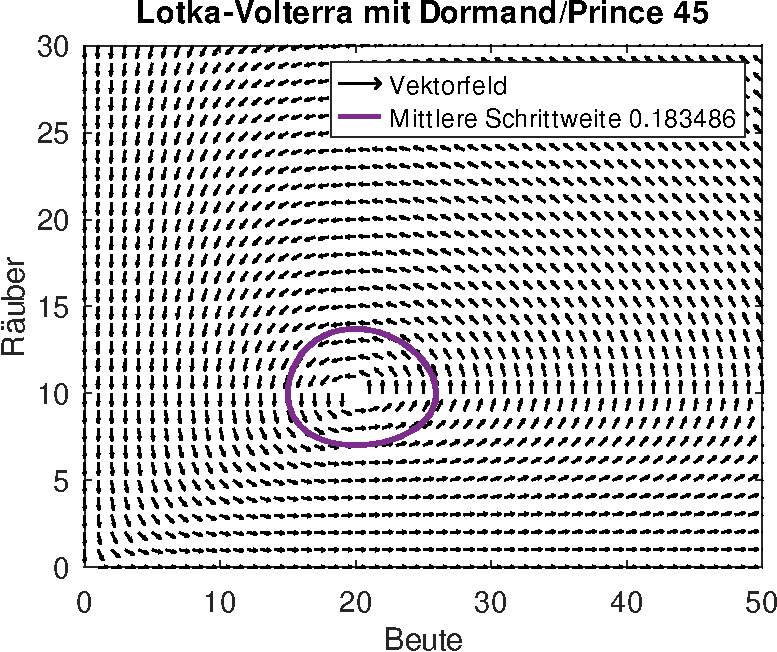
\includegraphics[width=.7\textwidth]{fig/DP45-LV-crop.pdf}}
    \only<2>{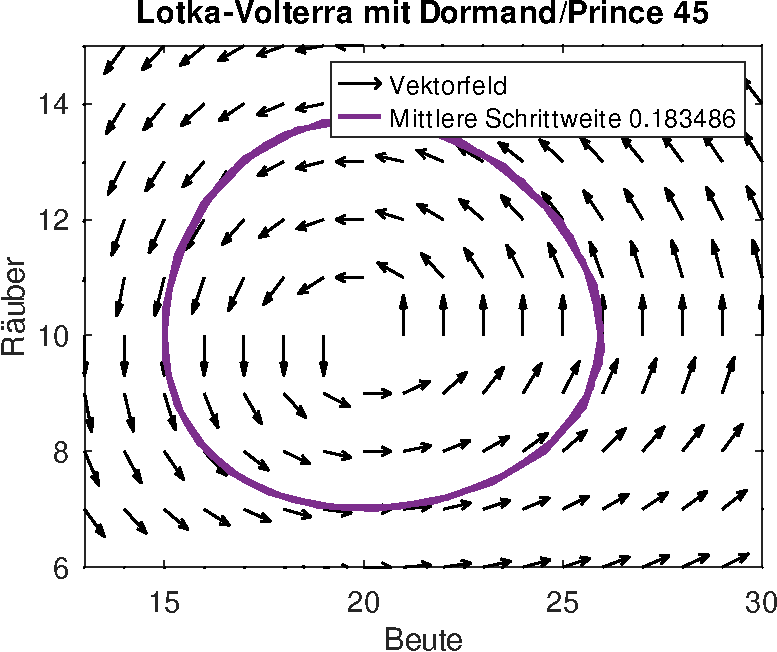
\includegraphics[width=.7\textwidth]{fig/DP45-LV-zoom-crop.pdf}}
  \end{center}
\end{frame}

\begin{frame}{Zusammenfassung}
  \begin{itemize}
  \item Zeitschrittverfahren bestehen aus zwei Teilen
    \begin{itemize}
    \item Zerlegung des Zeitintervalls in kleine Schritte
    \item Approximation der Vollterra-Integralgleichung auf jedem
      Teilintervall durch eine berechenbare Verfahrensfunktion
    \end{itemize}
    \item Die Genauigkeit der Lösung ist bestimmt durch
      \begin{itemize}
      \item die Wahl der Verfahrensfunktion
      \item die Schrittweite
      \end{itemize}
  \end{itemize}
\end{frame}
%%% Local Variables:
%%% mode: latex
%%% TeX-master: "slides.tex"
%%% End:
